\section{The \pktlanguage compiler}
\label{s:compiler}

\begin{figure*}[!t]
  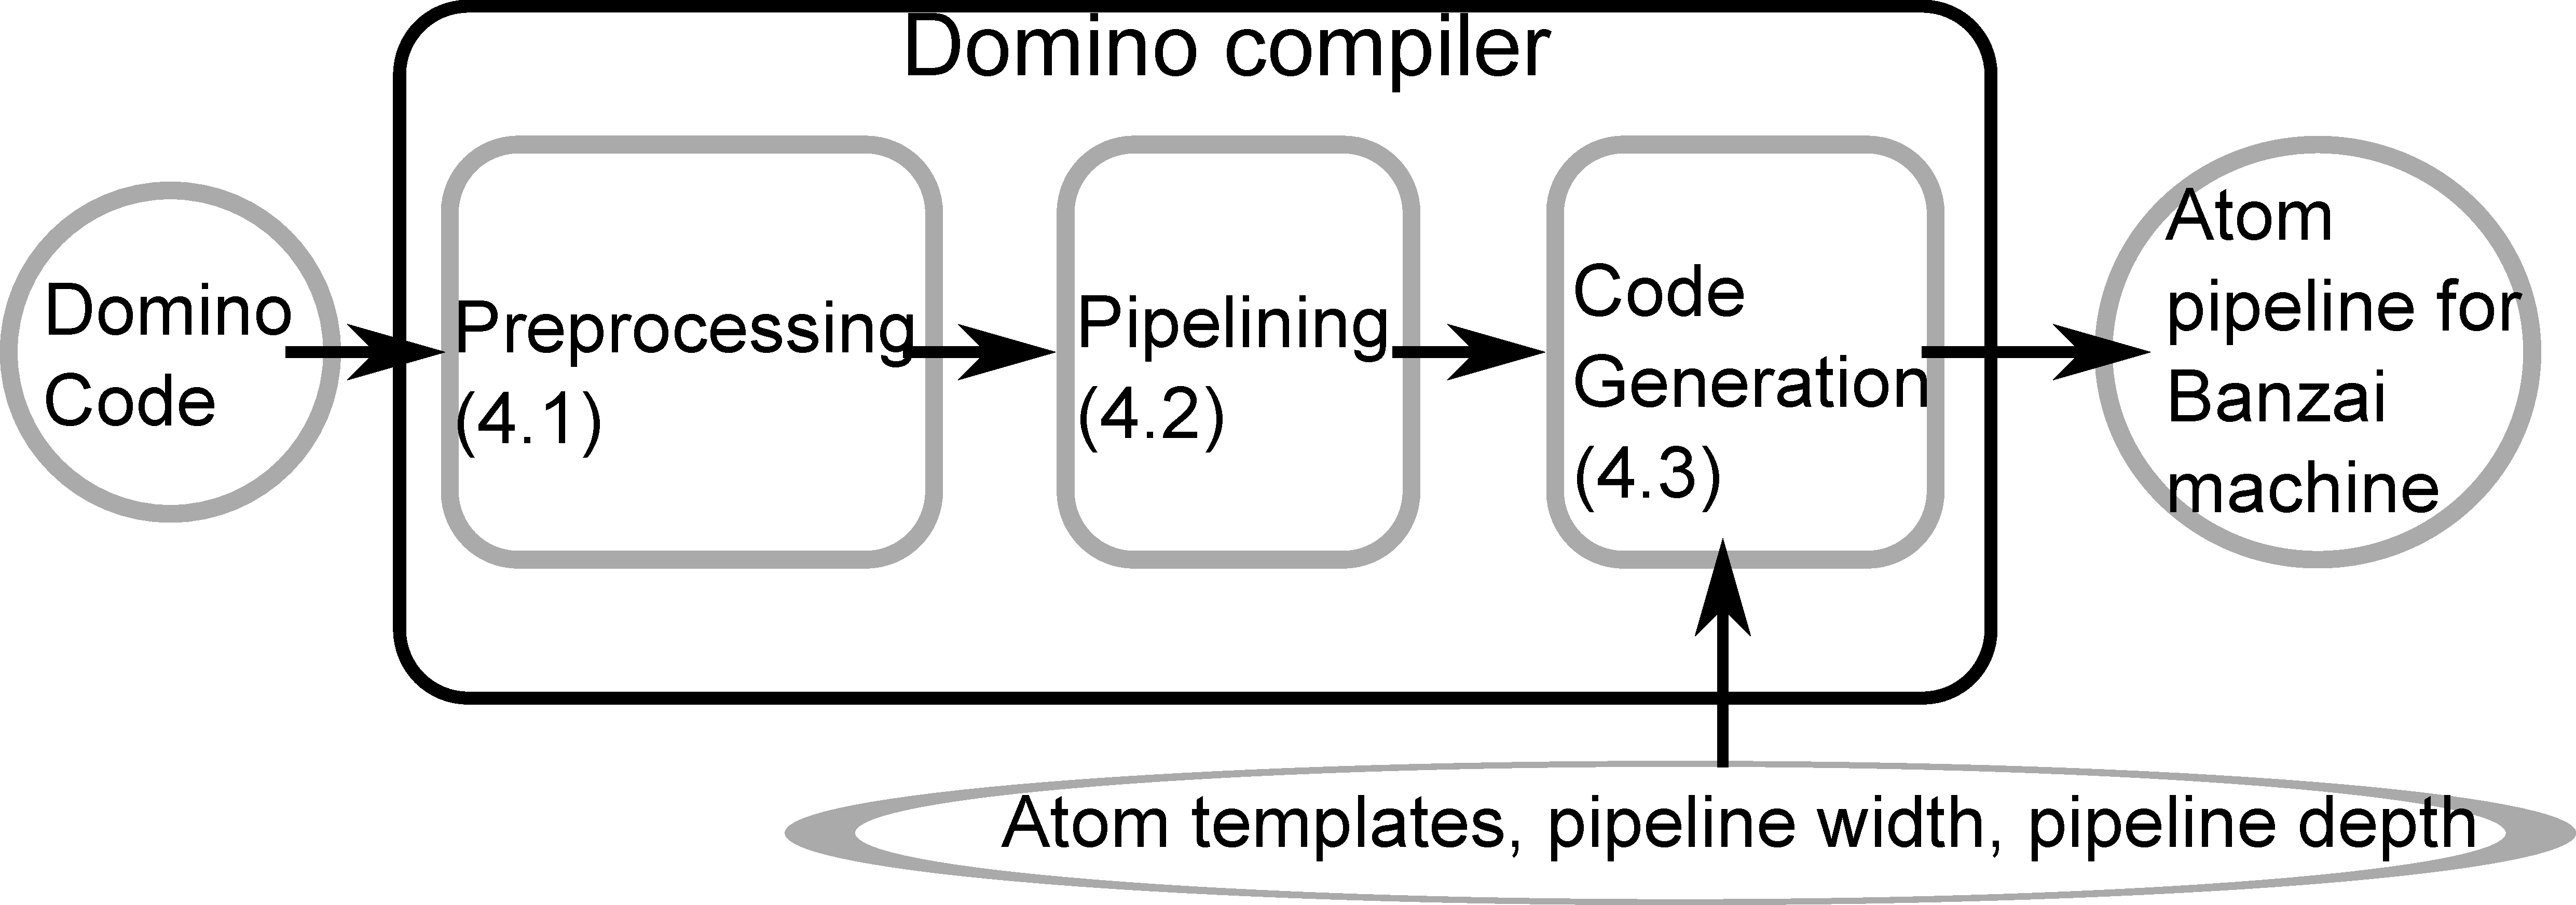
\includegraphics[width=\textwidth]{compiler.pdf}
  \caption{Passes in the \pktlanguage compiler}
\end{figure*}

We now describe the \pktlanguage compiler. We borrow several well-established
techniques from the compiler literature~\cite{muchnik}. However, as we show
throughout this section, constraining \pktlanguage for deterministic
performance has a happy side effect: it allows us to considerably simplify the
\pktlanguage compiler relative to mainstream compilers.

\subsection{Lexing, parsing, and semantic analysis}
Because \pktlanguage's syntax is based on C, we use clang's library
interface~\cite{libclang} to generate an Abstract Syntax Tree (AST) for a
packet transaction written in \pktlanguage. The remaining compiler passes
operate on this AST. Basing \pktlanguage's syntax on C has several benefits.
Clang's lexer and parser catch several errors with no additional effort. Using
C also allows us to use the macro preprocessor for constants. Finally,
intrinsic functions representing hardware primitives (e.g.  hashes and
checksum), can be implemented using arbitrary C code and linked with
\pktlanguage code before running the resulting binary on our abstract machine
(\S\ref{ss:verification}).

\subsection{If-conversion to straight-line code}
A packet transaction's body can contain if-else statements that alter the
program's control flow and complicate dependence analysis. We eliminate if-else
statements by transforming them into the C conditional operator, starting from
the innermost if statements and recursing outwards
(Figure~\ref{fig:if_convert}). This procedure is called
if-conversion~\cite{if_conversion}, but is much simpler in \pktlanguage because
only the if and else constructs alter control flow in \pktlanguage and all
other forms of control transfers (break, continue, loops) are forbidden.
\begin{figure*}[!t]
  \begin{minipage}{0.47\textwidth}
  \begin{small}
  \begin{lstlisting}[style=customc]
if (pkt.arrival -
    last_time[pkt.id] >
    THRESHOLD) {
 saved_hop[pkt.id] = pkt.new_hop;
}
  \end{lstlisting}
  \end{small}
  \end{minipage}
  \begin{minipage}{0.53\textwidth}
  \begin{small}
  \begin{lstlisting}[style=customc]
pkt.tmp = pkt.arrival -
          last_time[pkt.id]
          > THRESHOLD;
saved_hop[pkt.id] = pkt.tmp ?
                    pkt.new_hop :
                    saved_hop[pkt.id];
  \end{lstlisting}
  \end{small}
  \end{minipage}
\caption{Conversion to straight-line code}
\label{fig:if_convert}
\end{figure*}

This transformation creates straight-line code, where control always passes
sequentially without branching. Straight-line code simplifies
the rest of the compiler, as we will show (\S\ref{ss:ssa}).

\subsection{Converting state variables to load/store form}

We next identify all state variables used in a packet transaction, both arrays
and scalars, such as \texttt{last\_time} and \texttt{saved\_hop} in
Figure~\ref{fig:flowlet}. For each state variable, we create a \textit{read
flank} to read the state variable into a temporarily created packet field. For
an array, we also move the index expression into the read flank. Here, we
exploit the fact that only one array address is accessed by each packet in all
valid \pktlanguage programs.  We then replace all occurences of the state
variable with the packet temporary, and create a \textit{write flank} that
writes the packet temporary back into the state variable.  Figure
~\ref{fig:stateful_flanks} illustrates this transformation on a fragment.

\begin{figure*}[!t]
  \begin{minipage}{0.47\textwidth}
  \begin{small}
  \begin{lstlisting}[style=customc]
pkt.id = hash2(pkt.sport,
               pkt.dport)
         % NUM_FLOWLETS;
last_time[pkt.id] = pkt.arrival;
  \end{lstlisting}
  \end{small}
  \end{minipage}
  \begin{minipage}{0.53\textwidth}
  \begin{small}
  \begin{lstlisting}[style=customc]
// Read flank for last_time
pkt.id = hash2(pkt.sport,
                pkt.dport)
         % NUM_FLOWLETS;
pkt.last_time = last_time[pkt.id];

pkt.last_time = pkt.arrival;

// Write flank for last_time
last_time[pkt.id] = pkt.last_time;
  \end{lstlisting}
  \end{small}
  \end{minipage}
  \caption{Adding read and write flanks}
\label{fig:stateful_flanks}
\end{figure*}

After this pass, the code resembles code for a load-store
architecture~\cite{load_store}: state variables are only accessed through reads
and writes, and all arithemtic happens on packet variables. Restricting the
operations on state variables simplifies handling of state variables during
code partitioning (\S\ref{ss:partitioning}).

\subsection{Renaming variables to static single-Assignment Form}
We next convert to static single-assignment form (SSA)~\cite{ssa}, an
intermediate form used by many compilers~\cite{tree_ssa, llvm}.  In SSA, every
variable is assigned exactly once. To compute the SSA, we replace every
definition of a packet variable with a new packet variable and propagate this
new packet variable until the next definition of the same variable. State
variables are already in SSA form because after their flanks have been added,
every state variable is written exactly once in the wrie flank.  While general
algorithms to compute SSA are fairly involved~\cite{ssa}, \pktlanguage's SSA
computation is much simpler because it operates on straight-line code.

SSA simplifies further analysis. Because every variable is assigned exactly
once, there are no Write-After-Read or Write-After-Write dependencies; only
Read-After-Write dependencies remain. This, in turn, facilitates dependency
analysis during code partitioning (\S\ref{ss:partitioning}).

\begin{figure*}[!t]
  \begin{minipage}{0.48\textwidth}
  \begin{small}
  \begin{lstlisting}[style=customc]
pkt.id = hash2(pkt.sport,
               pkt.dport)
               % NUM_FLOWLETS;
pkt.last_time = last_time[pkt.id];
pkt.last_time = pkt.arrival;
last_time[pkt.id] = pkt.last_time;
  \end{lstlisting}
  \end{small}
  \end{minipage}
  \begin{minipage}{0.52\textwidth}
  \begin{small}
  \begin{lstlisting}[style=customc]
pkt.id0 = hash2(pkt.sport,
                pkt.dport)
                % NUM_FLOWLETS;
pkt.last_time0 = last_time[pkt.id0];
pkt.last_time1 = pkt.arrival;
last_time[pkt.id0] = pkt.last_time1;
  \end{lstlisting}
  \end{small}
  \end{minipage}
  \caption{SSA transformation}
\label{fig:ssa}
\end{figure*}

\subsection{Expression flattening to three-address code}
We next transform into three-address code, where all instructions are either
reads / writes into stateful variables or carry out packet manipulations of the
form: \texttt{pkt.f1 = pkt.f2 op pkt.f3;} where \texttt{op} includes all
arithmetic, logical, and relational operators. We also allow either pkt.f2 or
pkt.f3 to be an intrinsic function call, because we assume these are supported
in hardware. Three-address code instructions are similar to P4's action
primitives~\cite{p4spec} and RMT's VLIW instruction set~\cite{rmt}. To generate
three-address code, we flatten expressions that are not already legal
three-address code, by introducing enough temporaries
(Figure~\ref{fig:three_address}).

\begin{figure*}
\begin{lstlisting}[style=customc]
pkt.id            = hash2(pkt.sport, pkt.dport) % NUM_FLOWLETS;
pkt.saved_hop     = saved_hop[pkt.id]; @\label{line:stateRead}@
pkt.last_time     = last_time[pkt.id];
pkt.new_hop       = hash3(pkt.sport, pkt.dport, pkt.arrival) % NUM_HOPS;
pkt.tmp           = pkt.arrival - pkt.last_time;
pkt.tmp2          = pkt.tmp > THRESHOLD;
pkt.next_hop      = pkt.tmp2 ? pkt.new_hop : pkt.saved_hop;
saved_hop[pkt.id] = pkt.tmp2 ? pkt.new_hop : pkt.saved_hop; @\label{line:stateWrite}@
last_time[pkt.id] = pkt.arrival;
\end{lstlisting}
\caption{Flowlet switching in three-address code}
\label{fig:three_address}
\end{figure*}

\subsection{Code partitioning to codelets}
\label{ss:partitioning}
At this point, the code is still in sequential form. Code partitioning turns
sequential code into a pipeline of \textit{codelets}, where each codelet is a
small sequential block of three-address code statements. We generate this
pipeline of codelets, by exploiting parallelism within and across pipeline
stages. Subsequently, we map each codelets one-to-one to atoms provided by a
particular \absmachine instance~(\S\ref{ss:code_gen}), returning a compiler
error if any codelet doesn't map to an atom provided by the hardware.

To partition code into codelets, we carry out the following steps:
\begin{CompactEnumerate}
  \item Create a node for each statement (Figure~\ref{fig:three_address}) in
    the packet transaction after expression flattening.
  \item Create a bidrectional edge between N1 and N2 where N1 is a read from a
    state scalar / state array and N2 is a write into the same state scalar /
    state array. This step captures the constraint that state is internal to an
    atom in \absmachine. Because state variables don't occur in any
    instructions besides reads and writes, this step is all we need to handle
    state variables.
  \item Create an edge (N1, N2) for every pair of nodes N1, N2 where N2 reads
    a variable written by N1. We only check read-after-write dependencies because
    control dependencies turn into data dependencies when generating straight-line
    code. Further, the use of SSA removes all write-after-read and write-after-write
    dependencies.
  \item Generate strongly connected components (SCCs) of the resulting graph
    (Figure~\ref{fig:deps}) and condense the SCCs to to create a directed
    acyclic graph (DAG) (Figure~\ref{fig:dag}). This step captures the
    constraint that all operations on state variables (read, write, and modify)
    must reside within the same atom because state is local to an atom.
  \item Schedule the resulting DAG using critical path
    scheduling~\cite{crit_path_sched}, creating a new pipeline stage everytime
    one operation needs to follow another (Figure~\ref{fig:pipeline}).
\end{CompactEnumerate}

At this point, each node in Figure~\ref{fig:dag} can be turned into an codelet
and the resulting codelet pipeline (Figure~\ref{pipeline}) implements the
packet transaction.  Further, the codelets themselves have a stylized form.
Codelets that don't manipulate state contain exactly one three-address code
instruction. Codelets that manipulate state contain at least two statements: a
read from a state variable and a write to a state variable and optionally
consist of one or more updates to the state variable through packet
temporaries.

\begin{figure*}[!t]
\begin{minipage}{0.5\textwidth}
  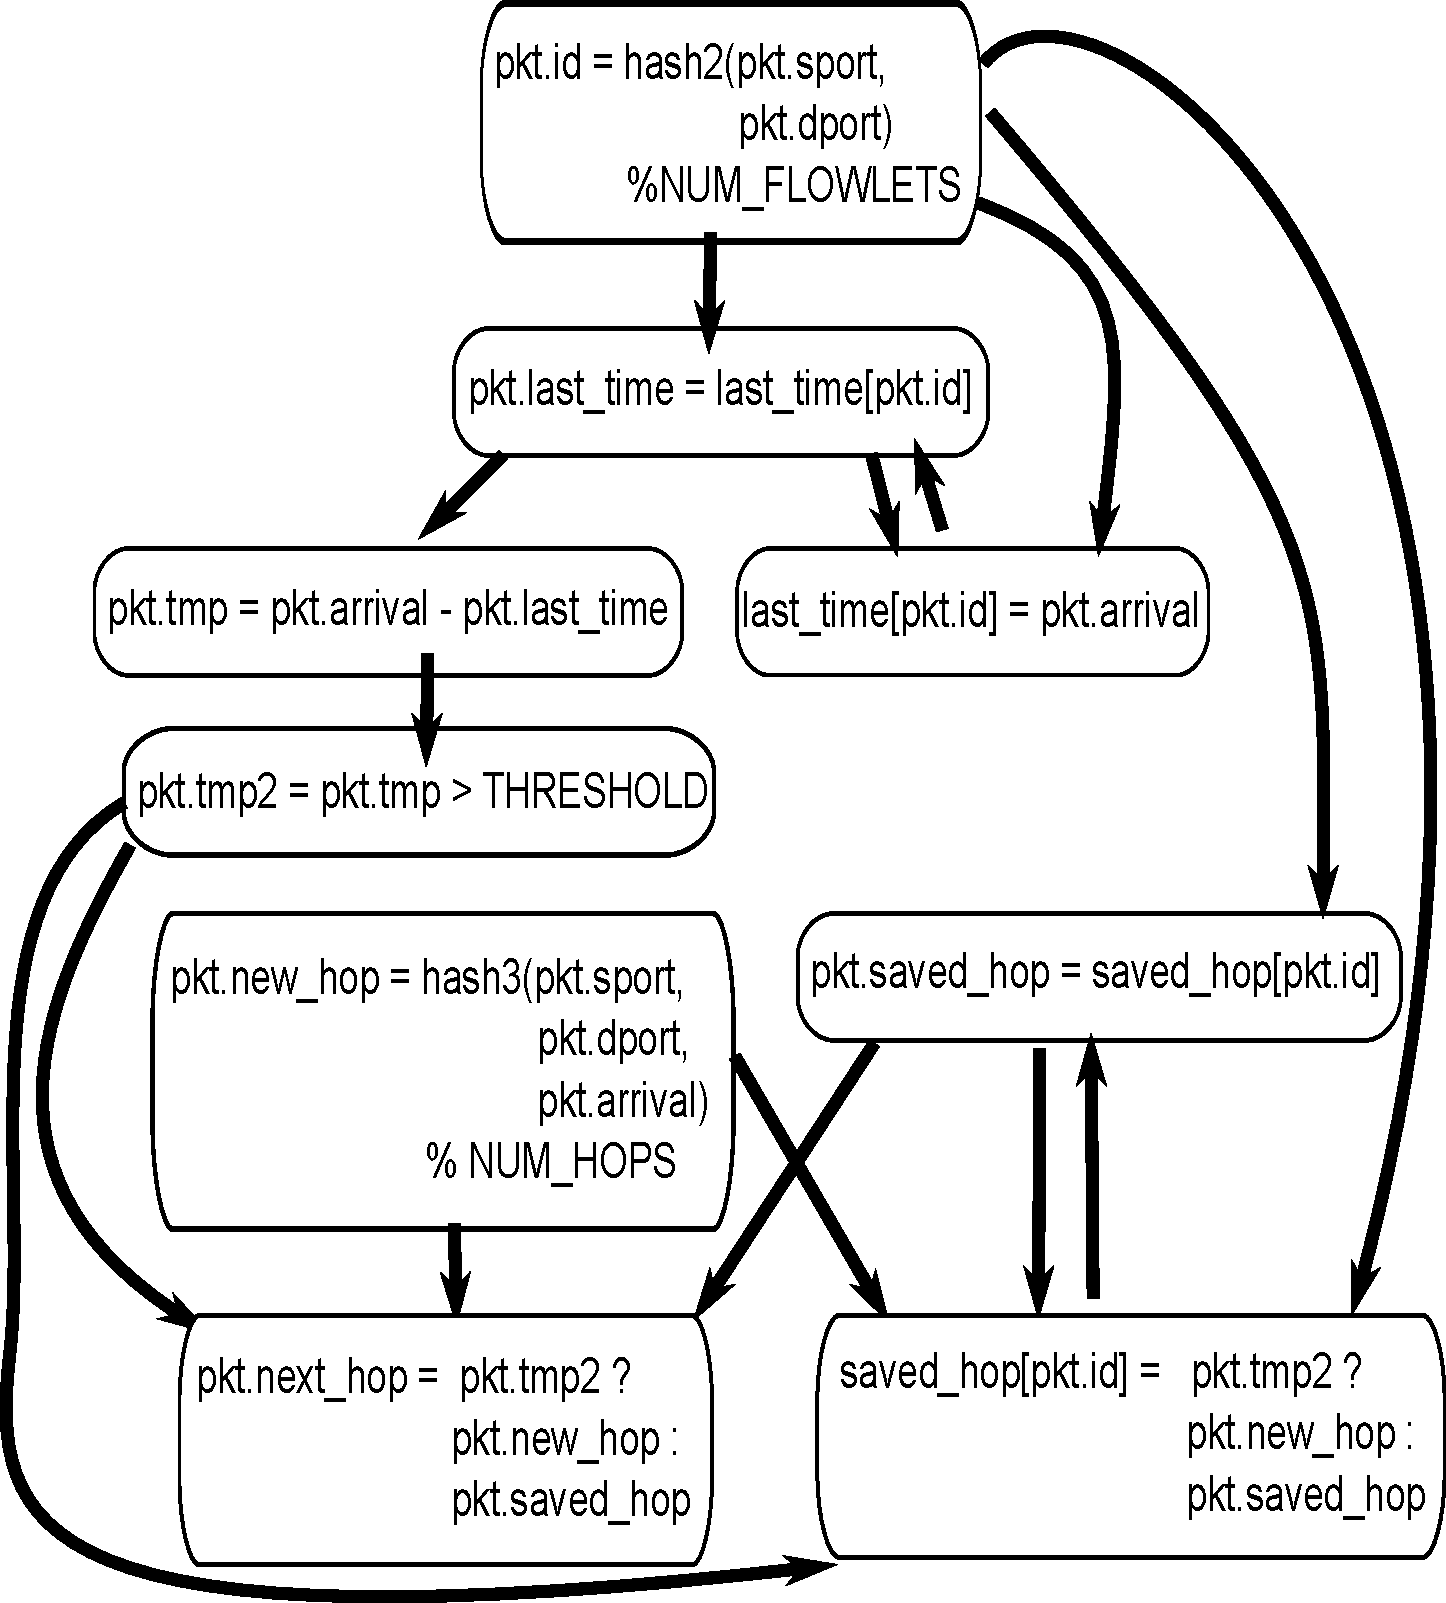
\includegraphics[width=\columnwidth]{deps.pdf}
\end{minipage}
%
\vrule\quad
%
\begin{minipage}{0.5\textwidth}
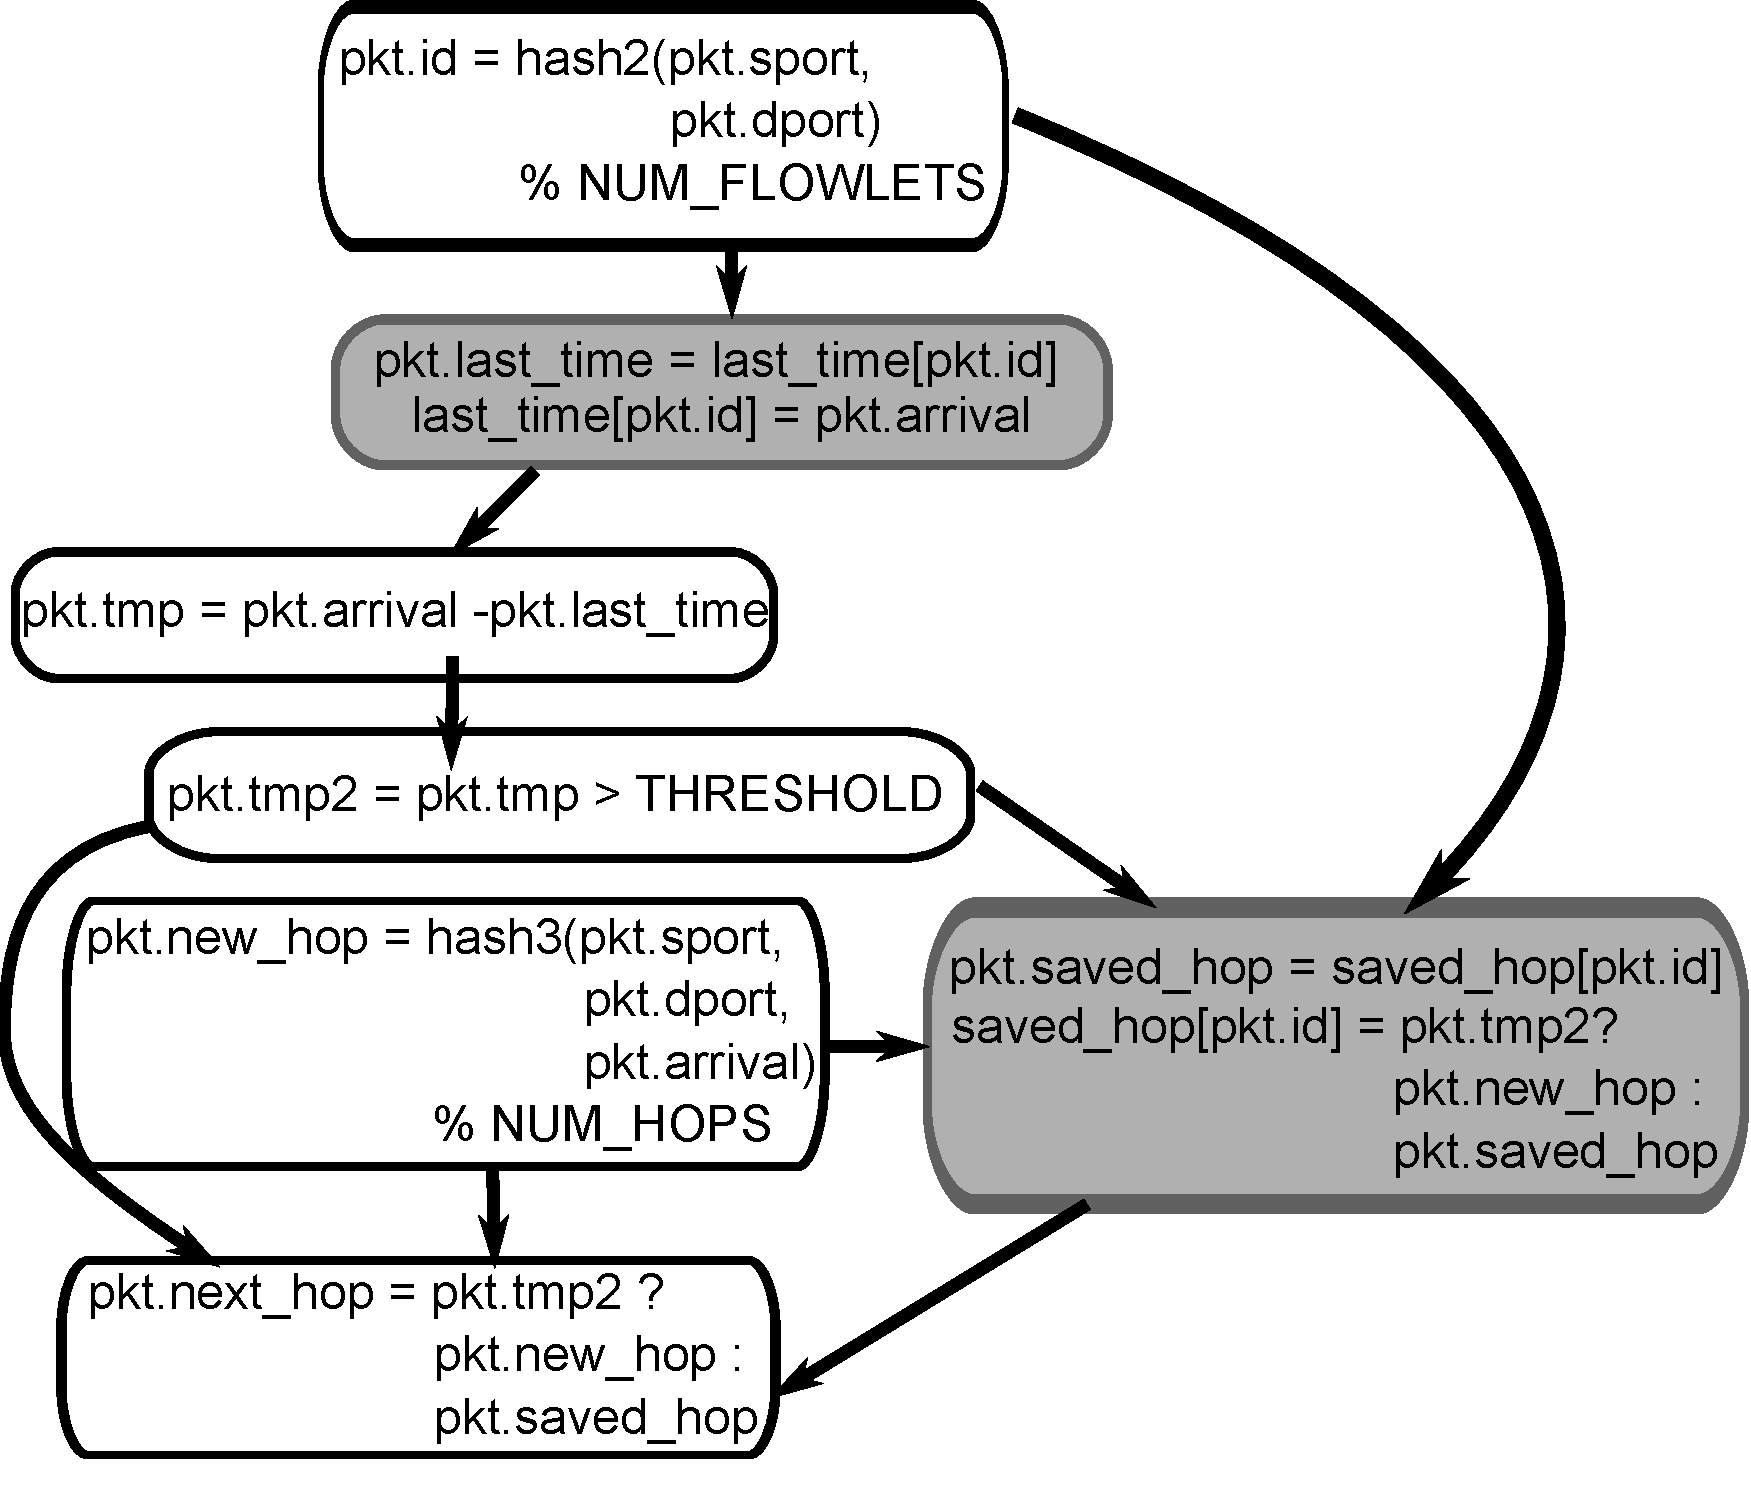
\includegraphics[width=\columnwidth]{scc.pdf}
\end{minipage}
\caption{Dependency graph before and after condensing strongly connected components}
\label{fig:partitioning}
\end{figure*}

% TODO: Like Alvin said, mention somewhere that SKETCH is a bounded checker
\subsection{Mapping a codelet to an atom}
\label{ss:complexity}
Next, we determine how the codelets created by code partitioning in the
previous step map one-to-one to atoms provided by the \absmachine instance. We
consider codelets that do and don't manipulate state separately because we
follow a different approach for each of them.

%TODO: Alvin can you read this and check if it makes sense?
\paragraph{Stateless codelets}
Expression flattening generates stateless codelets that each have only one
instruction in three-address code form (e.g. any of the unshaded boxes in
Figure~\ref{fig:pipeline}). For this paper, we will assume that all \absmachine
instances support all atoms that correspond to a single statement in
three-address code form. This assumption is backed by the fact that P4's
primitives~\cite{p4spec} and RMT's VLIW action set both contain instructions
that are in three-address code form. With this assumption, mapping a stateless
codelet to an atom is trivial: each stateless codelet has exactly one
three-address code instruction that is equivalent to an atom available in the
\absmachine instance.

If the \absmachine instance supported more complex atoms besides three-address
code instructions, then our approach is still correct, although suboptimal. For
instance, let us assume the \absmachine instance supports a
multiply-and-accumulate atom that multiplies a packet field by a constant, adds
another a packet field to it and then writes the result into a third packet
field. Then, our approach of flattening expressions would generate two codelets
(and hence two atoms): one to multiply and one to accumulate, where one atom
would have sufficed.

\paragraph{Stateful codelets}
Codelets that manipulate state have multi-line bodies that need to execute
atomically, and it is not readily apparent whether these codelets can be mapped
to an available atom. For instance, the update to the state variable
\texttt{saved\_hop} requires a read, followed by a write that perfoms a
conditional update. We develop a general technique to determine the
implementability of such stateful codelets, given as input the stateful atom
template provided by the underlying \absmachine instance.

We first state our problem more formally: the codelet is a specification that
needs to be implemented by searching over all possible candidates permitted by
the atom template.  More generally, we are looking for a way to
\textit{synthesize} the atom's \textit{configuration}, given an \textit{atom
template} describing the atom's functionality.

This is the realm of syntax-guided program synthesis~\cite{sgsyn} where the
programmer supplies a partial program (hence the term syntax-guided) with
missing details, and a specification. A program synthesis tool then fills in
these details in the partial program to ensure it matches up with the
specification. For instance, the SKETCH~\cite{bitstreaming, finite,
sketch_manual} compiler, an example of this approach, allows the programmer to
specify a partial program with \textit{holes} that are then ``filled in'' by
SKETCH to match a desired specification.

%TODO: Throw in a figure of the ALU.
We use SKETCH to solve the atom configuration problem as follows. Consider an
atom template that models an ALU (Figure~\ref{fig:alu}) taking two
configuration parameters: an opcode specifying an addition or subtraction
operation, and a 16-bit positive constant.  The ALU's functionality is to then
add or subtract this constant from one state variable. In SKETCH, the atom
template for this ALU would be represented as:
\begin{lstlisting}
bit choice = ??(1);
int constant = ??(16);
if (bit) {
  x = x + constant;
} else {
  x = x - constant;
}
\end{lstlisting}
where each ``??(n)'' represents a hole that can take values in $[0, 2^n -1]$.

The codelet that needs to be mapped to this atom (say x = x + 1, where x is a
state variable) can be fed into SKETCH as the desired specification
(Figure~\ref{fig:sketch_workflow}). SKETCH will then configure the atom
template by setting \texttt{choice} to 0 and \texttt{constant} to 1. If, on the
other hand, the codelet x = x * x was supplied as the SKETCH specification,
SKETCH would return an error because the specification cannot be synthesized by
the atom template.

Using SKETCH to represent atom templates allows us to express diverse atom
templates (\S\ref{\s:eval}) using a common imperative syntax. Because different
\absmachine instances only differ in the atom templates they provide, using
SKETCH as a code generator allows us to build a retargetable
compiler~\cite{rcc} with little target-dependent work beyond specifying each
target's atom templates as partial programs in SKETCH.

\subsection{Verifying compilations}

To conclude, we describe our testing infrastructure to verify that the
compilation is correct i.e. the externally visible behavior of the packet
transaction (Figure~\ref{fig:flowlet}) is indistinguishable from its pipelined
implementation (Figure~\ref{fig:pipeline}). We verify correctness by feeding in
the same set of test packets to both the packet transaction and its
implementation and comparing the outputs from both programs on the set of
externally visible fields. To create test packets, we scan the packet
transaction and generate the set of all packet fields read from or written to
by the transaction. We then initialize each of these fields by sampling
uniformly from the space of all 32-bit signed integers.

To compare outputs from the packet transaction and its implementation, we track
renames that occur because of SSA. We compare each output field in the
transactional form with the last rename of the same output field in the
implementation. We then feed the same number of test packets to both the
specification and implementation and compare outputs at the end of the
pipeline. This allows to quickly ``spot check'' our compilations and was
instrumental in uncovering a few bugs in various compilation passes during
development.
